% !TeX root =  main.tex

\chapter{Polynomial and Rational Functions}

\section{Quadratic Functions}
\begin{definition}
  A function $f(x)=ax^2+bx+c$ with $a\ne 0$ is called a \textbf{quadratic function}. Its graph is called a \textbf{parabola}. By completing the square (let $h=-\dfrac{b}{2a}$ and $k=f(h)$), a quadratic function can written in the \textbf{standard form} (or \textbf{vertex form}): $f(x)=a(x-h)^2+k$. The vertical line $x=-\dfrac{b}{2a}$ (or $x=h$) is called the \textbf{axis of symmetry}. The \textbf{vertex} $(h,k)$ is the intersection of the axis of symmetry and the parabola.
\end{definition}
\begin{note}
  The $y$-intercept of a quadratic function is $(0, f(0))$. The $x$-coordinates of $x$-intercepts are the zeros (or roots) of the function $f$, that is the solutions of the equation $f(x)=0$.
\end{note}

\begin{example}
  Find the vertex form of the quadratic function $f(x)=2 x^{2} + 4 x + 1$ and determine the vertex, axis of symmetry, $x$-intercepts, and $y$-intercept of the function.
\end{example}

\begin{note}
  \begin{itemize}
    \item A quadratic function $f(x)=ax^2+bx+c$ can be obtained from $y=x^2$ by a combination of vertical stretch by a factor $|a|$, a vertical reflection if $a<0$, a vertical shift of $f\left(-\frac{b}{2a}\right)$ units, and a horizontal shift of $-\frac{b}{2a}$ units.
    \item The domain of a quadratic function is $(-\infty, \infty)$.
    \item If $a>0$, then the parabola opens upward, the function has an absolute minimum $f\left(-\frac{b}{2a}\right)$, and the domain of the function is $[f\left(-\frac{b}{2a}\right), \infty)$.
    \item If $a<0$, then the parabola opens downward, the function has an absolute maximum $f\left(-\frac{b}{2a}\right)$, and the domain of the function is $(-\infty,f\left(-\frac{b}{2a}\right)]$.
  \end{itemize}
\end{note}
\newpage

\begin{example}
 Find the vertex form equation for the quadratic function $g$ in figure below as a transformation of $f(x)=x^2$, and then simplify the equation into general form.

 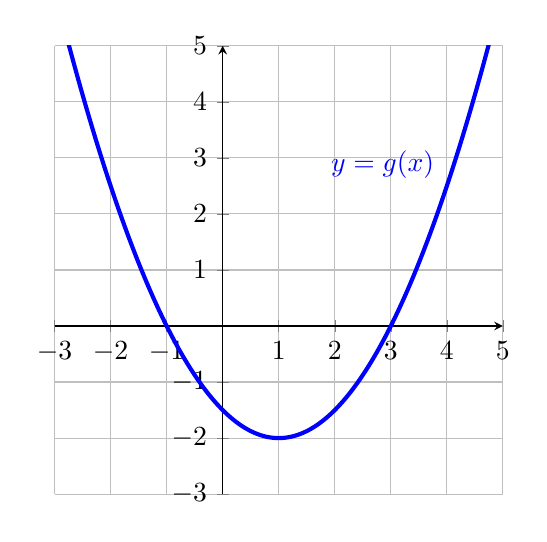
\begin{tikzpicture}
  \begin{axis}[
  axis lines=middle,
  unit vector ratio=1 1,
  ymajorgrids=true,
  xmajorgrids=true,
  xmin=-3,
  xmax=5,
  ymin=-3,
  ymax=5,
  xtick={-10,-9,...,10},
  ytick={-6,-5,...,6},]
  \addplot[blue, line width=1.5pt, smooth,samples=100,domain=-3:5] {1/2*(x-1)^2-2} node[pos=0.8, above left] {$y=g(x)$};
  \end{axis}
  \end{tikzpicture}
\end{example}

\begin{example}
  Find the domain and range of each function.\\
  \begin{enumerate*}
    \item $f(x)=3x^2+6x-5$.
    \item $f(x)=-2x^2+4-1$.\hfill\null
  \end{enumerate*}
\end{example}

\begin{example}
  A backyard farmer wants to enclose a rectangular space for a new garden within her fenced backyard. She has purchased 80 feet of wire fencing to enclose three sides, and she will use a section of the backyard fence as the fourth side.
\end{example}

\newpage

\begin{example}
  A local newspaper currently has 84,000 subscribers at a quarterly charge of \$30. Market research has suggested that if the owners raise the price to \$32, they would lose 5,000 subscribers. Assuming that subscriptions are linearly related to the price, what price should the newspaper charge for a quarterly subscription to maximize their revenue?
\end{example}

\begin{example}
  A ball is thrown upward from the top of a 40 foot high building at a speed of 80 feet per second. The ball's height above ground can be modeled by the equation \(H(t)=-16t^2+80t+40\).
\begin{enumerate}
  \item When does the ball reach the maximum height?
  \item What is the maximum height of the ball?  
  \item When does the ball hit the ground?
\end{enumerate}
\end{example}

\newpage

\section*{Exercise}

\begin{exercise}
  For each of the following functions,
  \begin{enumerate*}[label={()\alph*)}]
    \item $f(x)=x^2-4x+1$,
    \item $f(x)=-2x^2-4x+1$,\hfill\null
  \end{enumerate*}
  \begin{enumerate}
    \item write the function in vertex form,
    \item find the axis of symmetry,
    \item find the vertex,
    \item find the $y$-intercept,
    \item find the $x$-intercepts if they exist,
    \item find the domain and range,
    \item find the global maximum or minimum if it exist.
  \end{enumerate}
\end{exercise}

\begin{exercise}
  Find the vertex form equation for the quadratic function $f$ in figure below, and then simplify the equation into general form.
 
  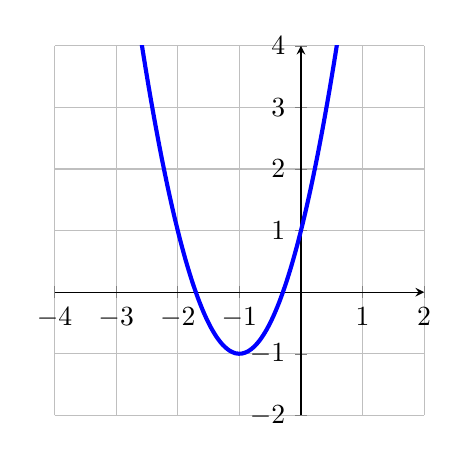
\begin{tikzpicture}
   \begin{axis}[
    width=0.6\textwidth,
   axis lines=middle,
   unit vector ratio=1 1,
   ymajorgrids=true,
   xmajorgrids=true,
   xmin=-4,
   xmax=2,
   ymin=-2,
   ymax=4,
   xtick={-10,-9,...,10},
   ytick={-6,-5,...,6},]
   \addplot[blue, line width=1.5pt, smooth,samples=100] {2*(x+1)^2-1} node[pos=0.2, right] {$y=f(x)$};
   \end{axis}
   \end{tikzpicture}
 \end{exercise}

\newpage

\begin{exercise}
  Find the dimensions of the rectangular parking lots producing the greatest area given that \(500\) feet of fencing will be used to for three sides.
\end{exercise}

\begin{exercise}
  A rocket is launched in the air. Its height, in meters above sea level, as a function of time, in seconds, is given by \(h(t)=-4.9t^2+229t+234\). Find the maximum height the rocket attains.
\end{exercise}

\begin{exercise}
  A soccer stadium holds \(62,000\) spectators. With a ticket price of \(\$11\), the average attendance has been \(26,000\). When the price dropped to \(\$9\), the average attendance rose to \(31,000\). Assuming that attendance is linearly related to ticket price, what ticket price would maximize revenue?
\end{exercise}

\newpage

\section{Power and Polynomial Functions}

\begin{definition}
  A \textbf{power function} is a function that can be represented in the form
\[f(x)=kx^p,\]
where \(k\) and \(p\) are real numbers, and \(k\) is known as the \textbf{coefficient}.
\end{definition}

\begin{example}
  Determine if the function is a power function.\\
  \begin{enumerate*}
    \item $f(x)=-2x^3$
    \item $f(x)=\dfrac{1}{x^2}$
    \item $f(x)=\sqrt[3]{x}$
    \item $f(x)=2^x$
    \item $f(x)=2x^2\cdot 3x^5$
    \item $f(x)=\dfrac{x}{x+1}$
  \end{enumerate*}
\end{example}

\begin{definition}
  The \textbf{end behavior} of a function $f$ is the general direction that the function $f$ approaches as $x$ goes to $\infty$ or $-\infty$. 
  
  We use an arrow $\to$ to describe ``goes to'' or ``approaches to''. 
  The notation $x\to \infty$ or $x\to -\infty$ means ``$x$ goes to infinity'' or ``$x$ goes to negative infinity'' respectively.
  The notation $f(x)\to \infty$ or $f(x)\to -\infty$ means ``$f(x)$ goes to infinity'' or ``$f(x)$ goes to negative infinity'' respectively.

  If $f(x)\to b$ as $x\to \infty$ or $x\to -\infty$, then we say the line $y=b$ is a \textbf{horizontal asymptote}.
\end{definition}

\begin{howto}
  To determine the end behavior of a function $f$, take a large positive number $N$. 
  
  If $f(N)$ is a large positive number, then $f(x)\to \infty$ as $x\to \infty$. 
  
  If $-f(N)$ is a large positive number, then $f(x)\to -\infty$ as $x\to \infty$.
  
  If $f(-N)$ is a large positive number, then $f(x)\to\infty$ as $x\to -\infty$. 
  
  If $-f(-N)$ is a large positive number, then $f(x)\to-\infty$ as $x\to -\infty$.
\end{howto}

\begin{example}
  Determine the end behavior(s) of the function.\\
  \begin{enumerate*}
    \item $f(x)=-2x^3$
    \item $f(x)=\dfrac{1}{x^2}$
    \item $f(x)=\sqrt[3]{x}$\hfill\null
  \end{enumerate*}
\end{example}

\newpage

\begin{definition}
  Let $n$ be a non-negative integer. A \textbf{polynomial function} of \textbf{degree} $n$ is a function that can be written in the form 
  \[f(x)=a_nx^n + \cdots + a_2x^2 + a_1x + a_0.\]
\begin{itemize}
  \item Each \(a_i\) is a \textbf{coefficient}. 
  \item Each product \(a_ix^i\) is a \textbf{term} of a polynomial function.
  \item The term $a_nx^n$ is called the \textbf{leading term}. The number $a_n$ is called the \textbf{leading coefficient}.
  \item The number $a_0$ is called the \textbf{constant term}.
\end{itemize}
\end{definition}

\begin{note}
  The end behavior of a polynomial function $f(x)=a_nx^2+\cdots +a_0$ of degree $n$ is completely determined by the end behavior of the power function $g(x)=a_nx^n$.
  
  The domain of a polynomial function is $(-\infty, \infty)$. The range of an odd degree polynomial function is also $(-\infty, \infty)$. The range of an even degree polynomial function is either $[y_\text{min}, \infty)$ if $a_n>0$ or $(-\infty, y_\text{max}]$ if $a_n<0$, where $y_\text{min}$ (respectively, $y_\text{max}$) is the absolute minimum (respectively, maximum) of the function. 
\end{note}

\begin{example}
  Determine the end behavior of the function.\\
  \begin{enumerate*}
    \item $f(x)=2x^4-3x+1$
    \item $g(x)=-3x^3+2x^2-x$
    \item $h(x)=-4x^6-7x^5+10x^4+2$\hfill\null
  \end{enumerate*}
\end{example}

\begin{example}
  Identify the degree, the leading therm and the end behavior of the polynomial function.\\
  \begin{enumerate*}
    \item $f(x)=-3x^2(x-1)(x+4)$
    \item $f(x)=2x^3(1-x)(x+1)$\hfill\null
  \end{enumerate*}
\end{example}

\newpage

\begin{definition}
  If $f$ is a polynomial function, then a number $c$ is called a \textbf{zero} of $f$ if $f(c)=0$.
\end{definition}

\begin{proposition}
  Let $f$ be a polynomial and $c$ a real number. Then the following are equivalent:
  \begin{enumerate}
    \item $c$ is a zero of $f$.
    \item $x=c$ is a solution of the equation $f(x)=0$.
    \item $x-c$ is a factor of $f(x)$.
    \item $(c,0)$ is an $x$-intercept of the function of $y=f(x)$.
  \end{enumerate}
\end{proposition}

\begin{example}
  Find $x$-intercepts and the $y$-intercept of the polynomial function $f(x)=x^{3} + 3 x^{2} - x - 3$.
\end{example}

\begin{example}
  Find $x$-intercepts and the $y$-intercept of the polynomial function $f(x)=x^4+2x^2-3$.
\end{example}

\begin{definition}
  A \textbf{continuous} function has no breaks in its graph. A \textbf{smooth} function is a continuous function whose graph that has no sharp corners.
\end{definition}
\begin{note}
  Polynomial functions are smooth functions.
\end{note}

\begin{theorem}[Intermediate Value Theorem for Polynomials]
If $f$ is a polynomial function and $f(a)f(b)<0$, then there exists at least one value $c$ between $a$ and $b$ such that $f(c)=0$.
\end{theorem}

\begin{corollary}
  Let $f$ be a polynomial function, $a$ and $b$ real zeros of $f$. If $f$ has no other zeros between $a$ and $b$, then either $f(x)>0$ for all $x$ between $a$ and $b$ or $f(x)<0$ for all $x$ between $a$ and $b$.
\end{corollary}

\newpage

\begin{example}
  Determine if the polynomial function $f(x)=5x^4-2x^3-20$ has a zero on the interval $[1, 2]$.
\end{example}

\begin{definition}
  A \textbf{turning point} is a point at which the function values change from increasing to decreasing or decreasing to increasing.
\end{definition}

\begin{theorem}[Fundamental Theorem of Algebra]
  A degree $n$ polynomial function has at least one complex zero.
\end{theorem}

\begin{proposition}
  A degree $n$ polynomial function may have at most $n$ real zeros and $n-1$ turning points.
\end{proposition}

\newpage

\begin{example}
  Consider the polynomial function  $f(x)=(x-2)(x+1)(x-4)$. Determine the zeros, the number of turning points, the $x$-intercepts, and the $y$-intercept.
\end{example}

\newpage

\begin{example}
  What can we conclude about the leading term of the polynomial function $y=f(x)$ represented by the graph below.\\
  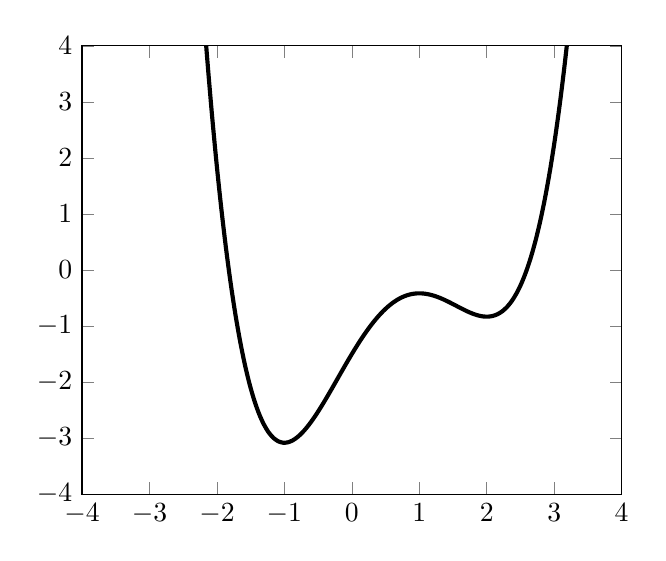
\begin{tikzpicture}
    \begin{axis}[
    xmin=-4,
    xmax=4,
    ymin=-4,
    ymax=4,
    xtick={-10,-9,...,10},
    ytick={-10,-9,...,10},]
    \addplot[line width=1.5pt, smooth, samples=100, domain=-3:4] {1/4*(x)^(4)-2/3*(x)^(3)-1/2*(x)^(2)+2*(x)-3/2} node[pos=0.9, left] {$y=f(x)$};
    \end{axis}
  \end{tikzpicture}
\end{example}
\vspace*{-0.4\textheight}


\newpage
\section{Graphs of Polynomial Functions}

\section{Dividing of Polynomials}

\section{Zeros of Polynomials}

\section{Rational Functions}

\section{Polynomial and Rational Inequalities}



